\documentclass[1p]{elsarticle_modified}
%\bibliographystyle{elsarticle-num}

%\usepackage[colorlinks]{hyperref}
%\usepackage{abbrmath_seonhwa} %\Abb, \Ascr, \Acal ,\Abf, \Afrak
\usepackage{amsfonts}
\usepackage{amssymb}
\usepackage{amsmath}
\usepackage{amsthm}
\usepackage{scalefnt}
\usepackage{amsbsy}
\usepackage{kotex}
\usepackage{caption}
\usepackage{subfig}
\usepackage{color}
\usepackage{graphicx}
\usepackage{xcolor} %% white, black, red, green, blue, cyan, magenta, yellow
\usepackage{float}
\usepackage{setspace}
\usepackage{hyperref}

\usepackage{tikz}
\usetikzlibrary{arrows}

\usepackage{multirow}
\usepackage{array} % fixed length table
\usepackage{hhline}

%%%%%%%%%%%%%%%%%%%%%
\makeatletter
\renewcommand*\env@matrix[1][\arraystretch]{%
	\edef\arraystretch{#1}%
	\hskip -\arraycolsep
	\let\@ifnextchar\new@ifnextchar
	\array{*\c@MaxMatrixCols c}}
\makeatother %https://tex.stackexchange.com/questions/14071/how-can-i-increase-the-line-spacing-in-a-matrix
%%%%%%%%%%%%%%%

\usepackage[normalem]{ulem}

\newcommand{\msout}[1]{\ifmmode\text{\sout{\ensuremath{#1}}}\else\sout{#1}\fi}
%SOURCE: \msout is \stkout macro in https://tex.stackexchange.com/questions/20609/strikeout-in-math-mode

\newcommand{\cancel}[1]{
	\ifmmode
	{\color{red}\msout{#1}}
	\else
	{\color{red}\sout{#1}}
	\fi
}

\newcommand{\add}[1]{
	{\color{blue}\uwave{#1}}
}

\newcommand{\replace}[2]{
	\ifmmode
	{\color{red}\msout{#1}}{\color{blue}\uwave{#2}}
	\else
	{\color{red}\sout{#1}}{\color{blue}\uwave{#2}}
	\fi
}

\newcommand{\Sol}{\mathcal{S}} %segment
\newcommand{\D}{D} %diagram
\newcommand{\A}{\mathcal{A}} %arc


%%%%%%%%%%%%%%%%%%%%%%%%%%%%%5 test

\def\sl{\operatorname{\textup{SL}}(2,\Cbb)}
\def\psl{\operatorname{\textup{PSL}}(2,\Cbb)}
\def\quan{\mkern 1mu \triangleright \mkern 1mu}

\theoremstyle{definition}
\newtheorem{thm}{Theorem}[section]
\newtheorem{prop}[thm]{Proposition}
\newtheorem{lem}[thm]{Lemma}
\newtheorem{ques}[thm]{Question}
\newtheorem{cor}[thm]{Corollary}
\newtheorem{defn}[thm]{Definition}
\newtheorem{exam}[thm]{Example}
\newtheorem{rmk}[thm]{Remark}
\newtheorem{alg}[thm]{Algorithm}

\newcommand{\I}{\sqrt{-1}}
\begin{document}

%\begin{frontmatter}
%
%\title{Boundary parabolic representations of knots up to 8 crossings}
%
%%% Group authors per affiliation:
%\author{Yunhi Cho} 
%\address{Department of Mathematics, University of Seoul, Seoul, Korea}
%\ead{yhcho@uos.ac.kr}
%
%
%\author{Seonhwa Kim} %\fnref{s_kim}}
%\address{Center for Geometry and Physics, Institute for Basic Science, Pohang, 37673, Korea}
%\ead{ryeona17@ibs.re.kr}
%
%\author{Hyuk Kim}
%\address{Department of Mathematical Sciences, Seoul National University, Seoul 08826, Korea}
%\ead{hyukkim@snu.ac.kr}
%
%\author{Seokbeom Yoon}
%\address{Department of Mathematical Sciences, Seoul National University, Seoul, 08826,  Korea}
%\ead{sbyoon15@snu.ac.kr}
%
%\begin{abstract}
%We find all boundary parabolic representation of knots up to 8 crossings.
%
%\end{abstract}
%\begin{keyword}
%    \MSC[2010] 57M25 
%\end{keyword}
%
%\end{frontmatter}

%\linenumbers
%\tableofcontents
%
\newcommand\colored[1]{\textcolor{white}{\rule[-0.35ex]{0.8em}{1.4ex}}\kern-0.8em\color{red} #1}%
%\newcommand\colored[1]{\textcolor{white}{ #1}\kern-2.17ex	\textcolor{white}{ #1}\kern-1.81ex	\textcolor{white}{ #1}\kern-2.15ex\color{red}#1	}

{\Large $\underline{10_{60}~(K10a_{1})}$}

\setlength{\tabcolsep}{10pt}
\renewcommand{\arraystretch}{1.6}
\vspace{1cm}\begin{tabular}{m{100pt}>{\centering\arraybackslash}m{274pt}}
\multirow{5}{120pt}{
	\centering
	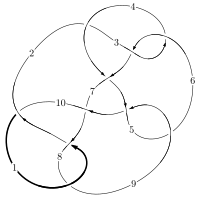
\includegraphics[width=112pt]{../../../GIT/diagram.site/Diagrams/png/144_10_60.png}\\
\ \ \ A knot diagram\footnotemark}&
\allowdisplaybreaks
\textbf{Linearized knot diagam} \\
\cline{2-2}
 &
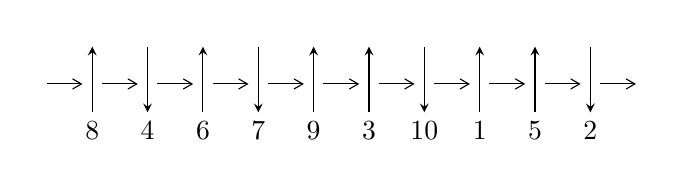
\begin{tikzpicture}[x=20pt, y=17pt]
	% nodes
	\node (C0) at (0, 0) {};
	\node (C1) at (1, 0) {};
	\node (C1U) at (1, +1) {};
	\node (C1D) at (1, -1) {8};

	\node (C2) at (2, 0) {};
	\node (C2U) at (2, +1) {};
	\node (C2D) at (2, -1) {4};

	\node (C3) at (3, 0) {};
	\node (C3U) at (3, +1) {};
	\node (C3D) at (3, -1) {6};

	\node (C4) at (4, 0) {};
	\node (C4U) at (4, +1) {};
	\node (C4D) at (4, -1) {7};

	\node (C5) at (5, 0) {};
	\node (C5U) at (5, +1) {};
	\node (C5D) at (5, -1) {9};

	\node (C6) at (6, 0) {};
	\node (C6U) at (6, +1) {};
	\node (C6D) at (6, -1) {3};

	\node (C7) at (7, 0) {};
	\node (C7U) at (7, +1) {};
	\node (C7D) at (7, -1) {10};

	\node (C8) at (8, 0) {};
	\node (C8U) at (8, +1) {};
	\node (C8D) at (8, -1) {1};

	\node (C9) at (9, 0) {};
	\node (C9U) at (9, +1) {};
	\node (C9D) at (9, -1) {5};

	\node (C10) at (10, 0) {};
	\node (C10U) at (10, +1) {};
	\node (C10D) at (10, -1) {2};
	\node (C11) at (11, 0) {};

	% arrows
	\draw[->,>={angle 60}]
	(C0) edge (C1) (C1) edge (C2) (C2) edge (C3) (C3) edge (C4) (C4) edge (C5) (C5) edge (C6) (C6) edge (C7) (C7) edge (C8) (C8) edge (C9) (C9) edge (C10) (C10) edge (C11) ;	\draw[->,>=stealth]
	(C1D) edge (C1U) (C2U) edge (C2D) (C3D) edge (C3U) (C4U) edge (C4D) (C5D) edge (C5U) (C6D) edge (C6U) (C7U) edge (C7D) (C8D) edge (C8U) (C9D) edge (C9U) (C10U) edge (C10D) ;
	\end{tikzpicture} \\
\hhline{~~} \\& 
\textbf{Solving Sequence} \\ \cline{2-2} 
 &
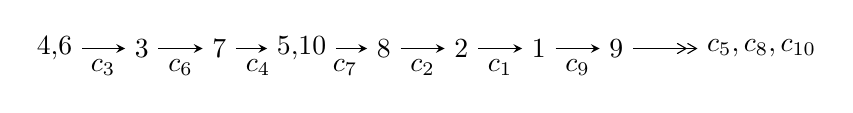
\begin{tikzpicture}[x=28pt, y=7pt]
	% node
	\node (A0) at (-1/8, 0) {4,6};
	\node (A1) at (1, 0) {3};
	\node (A2) at (2, 0) {7};
	\node (A3) at (49/16, 0) {5,10};
	\node (A4) at (33/8, 0) {8};
	\node (A5) at (41/8, 0) {2};
	\node (A6) at (49/8, 0) {1};
	\node (A7) at (57/8, 0) {9};
	\node (C1) at (1/2, -1) {$c_{3}$};
	\node (C2) at (3/2, -1) {$c_{6}$};
	\node (C3) at (5/2, -1) {$c_{4}$};
	\node (C4) at (29/8, -1) {$c_{7}$};
	\node (C5) at (37/8, -1) {$c_{2}$};
	\node (C6) at (45/8, -1) {$c_{1}$};
	\node (C7) at (53/8, -1) {$c_{9}$};
	\node (A8) at (9, 0) {$c_{5},c_{8},c_{10}$};

	% edge
	\draw[->,>=stealth]	
	(A0) edge (A1) (A1) edge (A2) (A2) edge (A3) (A3) edge (A4) (A4) edge (A5) (A5) edge (A6) (A6) edge (A7) ;
	\draw[->>,>={angle 60}]	
	(A7) edge (A8);
\end{tikzpicture} \\ 

\end{tabular} \\

\footnotetext{
The image of knot diagram is generated by the software ``\textbf{Draw programme}" developed by Andrew Bartholomew(\url{http://www.layer8.co.uk/maths/draw/index.htm\#Running-draw}), where we modified some parts for our purpose(\url{https://github.com/CATsTAILs/LinksPainter}).
}\phantom \\ \newline 
\centering \textbf{Ideals for irreducible components\footnotemark of $X_{\text{par}}$} 
 
\begin{align*}
I^u_{1}&=\langle 
u^{10}- u^9+3 u^8-2 u^7+3 u^6-2 u^5- u^2+b,\;u^{10}- u^9+4 u^8-3 u^7+6 u^6-4 u^5+3 u^4-2 u^3- u^2+a,\\
\phantom{I^u_{1}}&\phantom{= \langle  }u^{12}- u^{11}+4 u^{10}-3 u^9+7 u^8-5 u^7+6 u^6-4 u^5+2 u^4-2 u^3+u^2+1\rangle \\
I^u_{2}&=\langle 
- u^{33}+u^{32}+\cdots+b+1,\;- u^{32}+2 u^{31}+\cdots+a-2,\;u^{34}-2 u^{33}+\cdots-3 u+1\rangle \\
I^u_{3}&=\langle 
b+u,\;a,\;u^2+u+1\rangle \\
I^u_{4}&=\langle 
b+1,\;a,\;u^2+u+1\rangle \\
\\
\end{align*}
\raggedright * 4 irreducible components of $\dim_{\mathbb{C}}=0$, with total 50 representations.\\
\footnotetext{All coefficients of polynomials are rational numbers. But the coefficients are sometimes approximated in decimal forms when there is not enough margin.}
\newpage
\renewcommand{\arraystretch}{1}
\centering \section*{I. $I^u_{1}= \langle u^{10}- u^9+3 u^8-2 u^7+3 u^6-2 u^5- u^2+b,\;u^{10}- u^9+\cdots- u^2+a,\;u^{12}- u^{11}+\cdots+u^2+1 \rangle$}
\flushleft \textbf{(i) Arc colorings}\\
\begin{tabular}{m{7pt} m{180pt} m{7pt} m{180pt} }
\flushright $a_{4}=$&$\begin{pmatrix}1\\0\end{pmatrix}$ \\
\flushright $a_{6}=$&$\begin{pmatrix}0\\u\end{pmatrix}$ \\
\flushright $a_{3}=$&$\begin{pmatrix}1\\u^2\end{pmatrix}$ \\
\flushright $a_{7}=$&$\begin{pmatrix}u\\u^3+u\end{pmatrix}$ \\
\flushright $a_{5}=$&$\begin{pmatrix}u^4+u^2+1\\u^6+2 u^4+u^2\end{pmatrix}$ \\
\flushright $a_{10}=$&$\begin{pmatrix}- u^{10}+u^9-4 u^8+3 u^7-6 u^6+4 u^5-3 u^4+2 u^3+u^2\\- u^{10}+u^9-3 u^8+2 u^7-3 u^6+2 u^5+u^2\end{pmatrix}$ \\
\flushright $a_{8}=$&$\begin{pmatrix}u^{11}- u^{10}+3 u^9-2 u^8+3 u^7-2 u^6-2 u^3\\- u^9+u^8-3 u^7+2 u^6-3 u^5+2 u^4- u^3\end{pmatrix}$ \\
\flushright $a_{2}=$&$\begin{pmatrix}u^2+1\\u^2\end{pmatrix}$ \\
\flushright $a_{1}=$&$\begin{pmatrix}- u^{10}+u^9-4 u^8+3 u^7-6 u^6+4 u^5-4 u^4+2 u^3\\- u^{10}+u^9-3 u^8+2 u^7-3 u^6+2 u^5- u^4+u^2\end{pmatrix}$ \\
\flushright $a_{9}=$&$\begin{pmatrix}u^9- u^8+3 u^7-2 u^6+4 u^5-2 u^4+2 u^3\\u^{11}- u^{10}+4 u^9-3 u^8+6 u^7-4 u^6+4 u^5-2 u^4\end{pmatrix}$\\&\end{tabular}
\flushleft \textbf{(ii) Obstruction class $= -1$}\\~\\
\flushleft \textbf{(iii) Cusp Shapes $= 4 u^{11}-8 u^{10}+18 u^9-26 u^8+34 u^7-40 u^6+34 u^5-24 u^4+16 u^3-4 u^2+6 u-2$}\\~\\
\newpage\renewcommand{\arraystretch}{1}
\flushleft \textbf{(iv) u-Polynomials at the component}\newline \\
\begin{tabular}{m{50pt}|m{274pt}}
Crossings & \hspace{64pt}u-Polynomials at each crossing \\
\hline $$\begin{aligned}c_{1},c_{3},c_{6}\\c_{8}\end{aligned}$$&$\begin{aligned}
&u^{12}+u^{11}+4 u^{10}+3 u^9+7 u^8+5 u^7+6 u^6+4 u^5+2 u^4+2 u^3+u^2+1
\end{aligned}$\\
\hline $$\begin{aligned}c_{2},c_{10}\end{aligned}$$&$\begin{aligned}
&u^{12}+7 u^{11}+\cdots+2 u+1
\end{aligned}$\\
\hline $$\begin{aligned}c_{4},c_{7}\end{aligned}$$&$\begin{aligned}
&u^{12}- u^{11}+\cdots+2 u+1
\end{aligned}$\\
\hline $$\begin{aligned}c_{5},c_{9}\end{aligned}$$&$\begin{aligned}
&u^{12}-5 u^{11}+\cdots-12 u+4
\end{aligned}$\\
\hline
\end{tabular}\\~\\
\newpage\renewcommand{\arraystretch}{1}
\flushleft \textbf{(v) Riley Polynomials at the component}\newline \\
\begin{tabular}{m{50pt}|m{274pt}}
Crossings & \hspace{64pt}Riley Polynomials at each crossing \\
\hline $$\begin{aligned}c_{1},c_{3},c_{6}\\c_{8}\end{aligned}$$&$\begin{aligned}
&y^{12}+7 y^{11}+\cdots+2 y+1
\end{aligned}$\\
\hline $$\begin{aligned}c_{2},c_{10}\end{aligned}$$&$\begin{aligned}
&y^{12}- y^{11}+\cdots+6 y+1
\end{aligned}$\\
\hline $$\begin{aligned}c_{4},c_{7}\end{aligned}$$&$\begin{aligned}
&y^{12}-9 y^{11}+\cdots+2 y+1
\end{aligned}$\\
\hline $$\begin{aligned}c_{5},c_{9}\end{aligned}$$&$\begin{aligned}
&y^{12}+5 y^{11}+\cdots-16 y+16
\end{aligned}$\\
\hline
\end{tabular}\\~\\
\newpage\flushleft \textbf{(vi) Complex Volumes and Cusp Shapes}
$$\begin{array}{c|c|c}  
\text{Solutions to }I^u_{1}& \I (\text{vol} + \sqrt{-1}CS) & \text{Cusp shape}\\
 \hline 
\begin{aligned}
u &= -0.178968 + 0.877941 I \\
a &= -1.176440 - 0.426280 I \\
b &= -0.702552 + 0.572575 I\end{aligned}
 & -1.87720 - 1.89052 I & -4.24850 + 3.95054 I \\ \hline\begin{aligned}
u &= -0.178968 - 0.877941 I \\
a &= -1.176440 + 0.426280 I \\
b &= -0.702552 - 0.572575 I\end{aligned}
 & -1.87720 + 1.89052 I & -4.24850 - 3.95054 I \\ \hline\begin{aligned}
u &= \phantom{-}0.780097 + 0.281995 I \\
a &= \phantom{-}1.73075 + 0.13511 I \\
b &= \phantom{-}1.057890 + 0.528101 I\end{aligned}
 & -0.78013 - 3.73206 I & \phantom{-}3.21966 + 2.51013 I \\ \hline\begin{aligned}
u &= \phantom{-}0.780097 - 0.281995 I \\
a &= \phantom{-}1.73075 - 0.13511 I \\
b &= \phantom{-}1.057890 - 0.528101 I\end{aligned}
 & -0.78013 + 3.73206 I & \phantom{-}3.21966 - 2.51013 I \\ \hline\begin{aligned}
u &= -0.496677 + 1.117040 I \\
a &= -0.55633 + 2.12256 I \\
b &= \phantom{-}2.35694 + 1.72461 I\end{aligned}
 & -2.98532 - 7.52709 I & -1.88445 + 6.81034 I \\ \hline\begin{aligned}
u &= -0.496677 - 1.117040 I \\
a &= -0.55633 - 2.12256 I \\
b &= \phantom{-}2.35694 - 1.72461 I\end{aligned}
 & -2.98532 + 7.52709 I & -1.88445 - 6.81034 I \\ \hline\begin{aligned}
u &= \phantom{-}0.335900 + 1.207600 I \\
a &= -0.736004 - 0.940791 I \\
b &= \phantom{-}1.36295 - 1.08335 I\end{aligned}
 & -9.48086 + 3.21477 I & -6.88179 - 3.24710 I \\ \hline\begin{aligned}
u &= \phantom{-}0.335900 - 1.207600 I \\
a &= -0.736004 + 0.940791 I \\
b &= \phantom{-}1.36295 + 1.08335 I\end{aligned}
 & -9.48086 - 3.21477 I & -6.88179 + 3.24710 I \\ \hline\begin{aligned}
u &= \phantom{-}0.577185 + 1.164540 I \\
a &= \phantom{-}0.15978 - 1.92327 I \\
b &= \phantom{-}2.60480 - 1.08526 I\end{aligned}
 & -5.9276 + 13.9800 I & -2.44387 - 9.26853 I \\ \hline\begin{aligned}
u &= \phantom{-}0.577185 - 1.164540 I \\
a &= \phantom{-}0.15978 + 1.92327 I \\
b &= \phantom{-}2.60480 + 1.08526 I\end{aligned}
 & -5.9276 - 13.9800 I & -2.44387 + 9.26853 I\\
 \hline 
 \end{array}$$\newpage$$\begin{array}{c|c|c}  
\text{Solutions to }I^u_{1}& \I (\text{vol} + \sqrt{-1}CS) & \text{Cusp shape}\\
 \hline 
\begin{aligned}
u &= -0.517537 + 0.434237 I \\
a &= \phantom{-}1.57824 - 0.67661 I \\
b &= \phantom{-}0.319971 - 0.990159 I\end{aligned}
 & \phantom{-}1.31194 - 0.92364 I & \phantom{-}6.23895 + 2.73595 I \\ \hline\begin{aligned}
u &= -0.517537 - 0.434237 I \\
a &= \phantom{-}1.57824 + 0.67661 I \\
b &= \phantom{-}0.319971 + 0.990159 I\end{aligned}
 & \phantom{-}1.31194 + 0.92364 I & \phantom{-}6.23895 - 2.73595 I\\
 \hline 
 \end{array}$$\newpage\newpage\renewcommand{\arraystretch}{1}
\centering \section*{II. $I^u_{2}= \langle - u^{33}+u^{32}+\cdots+b+1,\;- u^{32}+2 u^{31}+\cdots+a-2,\;u^{34}-2 u^{33}+\cdots-3 u+1 \rangle$}
\flushleft \textbf{(i) Arc colorings}\\
\begin{tabular}{m{7pt} m{180pt} m{7pt} m{180pt} }
\flushright $a_{4}=$&$\begin{pmatrix}1\\0\end{pmatrix}$ \\
\flushright $a_{6}=$&$\begin{pmatrix}0\\u\end{pmatrix}$ \\
\flushright $a_{3}=$&$\begin{pmatrix}1\\u^2\end{pmatrix}$ \\
\flushright $a_{7}=$&$\begin{pmatrix}u\\u^3+u\end{pmatrix}$ \\
\flushright $a_{5}=$&$\begin{pmatrix}u^4+u^2+1\\u^6+2 u^4+u^2\end{pmatrix}$ \\
\flushright $a_{10}=$&$\begin{pmatrix}u^{32}-2 u^{31}+\cdots-3 u+2\\u^{33}- u^{32}+\cdots+2 u-1\end{pmatrix}$ \\
\flushright $a_{8}=$&$\begin{pmatrix}u^{12}+3 u^{10}+5 u^8-2 u^7+4 u^6-4 u^5+2 u^4-4 u^3+u^2+1\\- u^{33}+u^{32}+\cdots+3 u^2- u\end{pmatrix}$ \\
\flushright $a_{2}=$&$\begin{pmatrix}u^2+1\\u^2\end{pmatrix}$ \\
\flushright $a_{1}=$&$\begin{pmatrix}3 u^{32}-3 u^{31}+\cdots-6 u+4\\2 u^{33}+14 u^{31}+\cdots+2 u^3+u^2\end{pmatrix}$ \\
\flushright $a_{9}=$&$\begin{pmatrix}2 u^{32}-2 u^{31}+\cdots-3 u+2\\u^{33}+u^{32}+\cdots+u^2- u\end{pmatrix}$\\&\end{tabular}
\flushleft \textbf{(ii) Obstruction class $= -1$}\\~\\
\flushleft \textbf{(iii) Cusp Shapes $= -3 u^{33}+8 u^{32}-27 u^{31}+61 u^{30}-117 u^{29}+247 u^{28}-346 u^{27}+669 u^{26}-778 u^{25}+1328 u^{24}-1416 u^{23}+2034 u^{22}-2108 u^{21}+2492 u^{20}-2552 u^{19}+2536 u^{18}-2457 u^{17}+2183 u^{16}-1857 u^{15}+1579 u^{14}-1103 u^{13}+889 u^{12}-533 u^{11}+364 u^{10}-219 u^9+98 u^8-68 u^7+38 u^6-24 u^5+20 u^4-6 u^3+14 u^2-7 u+7$}\\~\\
\newpage\renewcommand{\arraystretch}{1}
\flushleft \textbf{(iv) u-Polynomials at the component}\newline \\
\begin{tabular}{m{50pt}|m{274pt}}
Crossings & \hspace{64pt}u-Polynomials at each crossing \\
\hline $$\begin{aligned}c_{1},c_{3},c_{6}\\c_{8}\end{aligned}$$&$\begin{aligned}
&u^{34}+2 u^{33}+\cdots+3 u+1
\end{aligned}$\\
\hline $$\begin{aligned}c_{2},c_{10}\end{aligned}$$&$\begin{aligned}
&u^{34}+16 u^{33}+\cdots+u+1
\end{aligned}$\\
\hline $$\begin{aligned}c_{4},c_{7}\end{aligned}$$&$\begin{aligned}
&u^{34}-2 u^{33}+\cdots-183 u+73
\end{aligned}$\\
\hline $$\begin{aligned}c_{5},c_{9}\end{aligned}$$&$\begin{aligned}
&(u^{17}+2 u^{16}+\cdots-5 u-2)^{2}
\end{aligned}$\\
\hline
\end{tabular}\\~\\
\newpage\renewcommand{\arraystretch}{1}
\flushleft \textbf{(v) Riley Polynomials at the component}\newline \\
\begin{tabular}{m{50pt}|m{274pt}}
Crossings & \hspace{64pt}Riley Polynomials at each crossing \\
\hline $$\begin{aligned}c_{1},c_{3},c_{6}\\c_{8}\end{aligned}$$&$\begin{aligned}
&y^{34}+16 y^{33}+\cdots+y+1
\end{aligned}$\\
\hline $$\begin{aligned}c_{2},c_{10}\end{aligned}$$&$\begin{aligned}
&y^{34}+4 y^{33}+\cdots+17 y+1
\end{aligned}$\\
\hline $$\begin{aligned}c_{4},c_{7}\end{aligned}$$&$\begin{aligned}
&y^{34}-8 y^{33}+\cdots-12903 y+5329
\end{aligned}$\\
\hline $$\begin{aligned}c_{5},c_{9}\end{aligned}$$&$\begin{aligned}
&(y^{17}+10 y^{16}+\cdots-23 y-4)^{2}
\end{aligned}$\\
\hline
\end{tabular}\\~\\
\newpage\flushleft \textbf{(vi) Complex Volumes and Cusp Shapes}
$$\begin{array}{c|c|c}  
\text{Solutions to }I^u_{2}& \I (\text{vol} + \sqrt{-1}CS) & \text{Cusp shape}\\
 \hline 
\begin{aligned}
u &= -0.723313 + 0.731528 I \\
a &= \phantom{-}0.151866 + 0.654346 I \\
b &= \phantom{-}0.514055 - 0.693038 I\end{aligned}
 & -0.85292 - 6.04614 I & -0.59802 + 7.72564 I \\ \hline\begin{aligned}
u &= -0.723313 - 0.731528 I \\
a &= \phantom{-}0.151866 - 0.654346 I \\
b &= \phantom{-}0.514055 + 0.693038 I\end{aligned}
 & -0.85292 + 6.04614 I & -0.59802 - 7.72564 I \\ \hline\begin{aligned}
u &= -0.624264 + 0.668207 I \\
a &= \phantom{-}0.475559 - 0.697137 I \\
b &= -0.299501 - 0.231577 I\end{aligned}
 & \phantom{-}1.18281 - 1.86595 I & \phantom{-}4.34837 + 4.33037 I \\ \hline\begin{aligned}
u &= -0.624264 - 0.668207 I \\
a &= \phantom{-}0.475559 + 0.697137 I \\
b &= -0.299501 + 0.231577 I\end{aligned}
 & \phantom{-}1.18281 + 1.86595 I & \phantom{-}4.34837 - 4.33037 I \\ \hline\begin{aligned}
u &= -0.575012 + 0.946029 I \\
a &= \phantom{-}0.488103 - 0.422358 I \\
b &= \phantom{-}0.267905 - 0.921351 I\end{aligned}
 & \phantom{-}0.36198 - 2.83643 I & \phantom{-}1.96538 + 0.68566 I \\ \hline\begin{aligned}
u &= -0.575012 - 0.946029 I \\
a &= \phantom{-}0.488103 + 0.422358 I \\
b &= \phantom{-}0.267905 + 0.921351 I\end{aligned}
 & \phantom{-}0.36198 + 2.83643 I & \phantom{-}1.96538 - 0.68566 I \\ \hline\begin{aligned}
u &= \phantom{-}0.839419 + 0.294756 I \\
a &= -2.21863 - 0.02513 I \\
b &= -1.75177 - 0.94314 I\end{aligned}
 & -3.32961 - 8.73955 I & \phantom{-}0.19211 + 5.92158 I \\ \hline\begin{aligned}
u &= \phantom{-}0.839419 - 0.294756 I \\
a &= -2.21863 + 0.02513 I \\
b &= -1.75177 + 0.94314 I\end{aligned}
 & -3.32961 + 8.73955 I & \phantom{-}0.19211 - 5.92158 I \\ \hline\begin{aligned}
u &= -0.678441 + 0.881986 I \\
a &= -0.269083 - 0.051645 I \\
b &= -1.117340 - 0.103610 I\end{aligned}
 & -1.29776 + 0.72905 I & -2.79971 - 1.68011 I \\ \hline\begin{aligned}
u &= -0.678441 - 0.881986 I \\
a &= -0.269083 + 0.051645 I \\
b &= -1.117340 + 0.103610 I\end{aligned}
 & -1.29776 - 0.72905 I & -2.79971 + 1.68011 I\\
 \hline 
 \end{array}$$\newpage$$\begin{array}{c|c|c}  
\text{Solutions to }I^u_{2}& \I (\text{vol} + \sqrt{-1}CS) & \text{Cusp shape}\\
 \hline 
\begin{aligned}
u &= \phantom{-}0.441434 + 1.051180 I \\
a &= -0.086124 - 0.253169 I \\
b &= -1.117340 - 0.103610 I\end{aligned}
 & -1.29776 + 0.72905 I & -2.79971 - 1.68011 I \\ \hline\begin{aligned}
u &= \phantom{-}0.441434 - 1.051180 I \\
a &= -0.086124 + 0.253169 I \\
b &= -1.117340 + 0.103610 I\end{aligned}
 & -1.29776 - 0.72905 I & -2.79971 + 1.68011 I \\ \hline\begin{aligned}
u &= -0.484889 + 1.050780 I \\
a &= \phantom{-}0.26211 - 1.43780 I \\
b &= -1.36154 - 1.18102 I\end{aligned}
 & -0.47242 - 3.20284 I & \phantom{-}2.38038 + 3.25895 I \\ \hline\begin{aligned}
u &= -0.484889 - 1.050780 I \\
a &= \phantom{-}0.26211 + 1.43780 I \\
b &= -1.36154 + 1.18102 I\end{aligned}
 & -0.47242 + 3.20284 I & \phantom{-}2.38038 - 3.25895 I \\ \hline\begin{aligned}
u &= -0.387508 + 1.102150 I \\
a &= \phantom{-}0.68089 + 1.93658 I \\
b &= \phantom{-}2.09444\phantom{ +0.000000I}\end{aligned}
 & -3.76357\phantom{ +0.000000I} & -3.71974 + 0. I\phantom{ +0.000000I} \\ \hline\begin{aligned}
u &= -0.387508 - 1.102150 I \\
a &= \phantom{-}0.68089 - 1.93658 I \\
b &= \phantom{-}2.09444\phantom{ +0.000000I}\end{aligned}
 & -3.76357\phantom{ +0.000000I} & -3.71974 + 0. I\phantom{ +0.000000I} \\ \hline\begin{aligned}
u &= \phantom{-}0.805751 + 0.171048 I \\
a &= -1.33086 + 0.63651 I \\
b &= -1.30277 + 0.63774 I\end{aligned}
 & -5.23887 - 0.57053 I & -2.63434 - 0.09683 I \\ \hline\begin{aligned}
u &= \phantom{-}0.805751 - 0.171048 I \\
a &= -1.33086 - 0.63651 I \\
b &= -1.30277 - 0.63774 I\end{aligned}
 & -5.23887 + 0.57053 I & -2.63434 + 0.09683 I \\ \hline\begin{aligned}
u &= \phantom{-}0.492477 + 1.076420 I \\
a &= \phantom{-}0.071402 + 0.579407 I \\
b &= \phantom{-}0.514055 + 0.693038 I\end{aligned}
 & -0.85292 + 6.04614 I & -0.59802 - 7.72564 I \\ \hline\begin{aligned}
u &= \phantom{-}0.492477 - 1.076420 I \\
a &= \phantom{-}0.071402 - 0.579407 I \\
b &= \phantom{-}0.514055 - 0.693038 I\end{aligned}
 & -0.85292 - 6.04614 I & -0.59802 + 7.72564 I\\
 \hline 
 \end{array}$$\newpage$$\begin{array}{c|c|c}  
\text{Solutions to }I^u_{2}& \I (\text{vol} + \sqrt{-1}CS) & \text{Cusp shape}\\
 \hline 
\begin{aligned}
u &= \phantom{-}0.276836 + 1.167190 I \\
a &= \phantom{-}0.004108 + 1.012990 I \\
b &= -1.30277 + 0.63774 I\end{aligned}
 & -5.23887 - 0.57053 I & -2.63434 - 0.09683 I \\ \hline\begin{aligned}
u &= \phantom{-}0.276836 - 1.167190 I \\
a &= \phantom{-}0.004108 - 1.012990 I \\
b &= -1.30277 - 0.63774 I\end{aligned}
 & -5.23887 + 0.57053 I & -2.63434 + 0.09683 I \\ \hline\begin{aligned}
u &= \phantom{-}0.242359 + 1.211260 I \\
a &= \phantom{-}0.12569 - 1.56340 I \\
b &= \phantom{-}1.50375 - 0.40483 I\end{aligned}
 & -8.21063 - 5.43973 I & -5.49430 + 3.57628 I \\ \hline\begin{aligned}
u &= \phantom{-}0.242359 - 1.211260 I \\
a &= \phantom{-}0.12569 + 1.56340 I \\
b &= \phantom{-}1.50375 + 0.40483 I\end{aligned}
 & -8.21063 + 5.43973 I & -5.49430 - 3.57628 I \\ \hline\begin{aligned}
u &= \phantom{-}0.556877 + 1.148560 I \\
a &= -0.15813 + 1.53835 I \\
b &= -1.75177 + 0.94314 I\end{aligned}
 & -3.32961 + 8.73955 I & \phantom{-}0.19211 - 5.92158 I \\ \hline\begin{aligned}
u &= \phantom{-}0.556877 - 1.148560 I \\
a &= -0.15813 - 1.53835 I \\
b &= -1.75177 - 0.94314 I\end{aligned}
 & -3.32961 - 8.73955 I & \phantom{-}0.19211 + 5.92158 I \\ \hline\begin{aligned}
u &= \phantom{-}0.520828 + 1.178390 I \\
a &= \phantom{-}0.76467 - 1.29488 I \\
b &= \phantom{-}1.50375 + 0.40483 I\end{aligned}
 & -8.21063 + 5.43973 I & -5.49430 - 3.57628 I \\ \hline\begin{aligned}
u &= \phantom{-}0.520828 - 1.178390 I \\
a &= \phantom{-}0.76467 + 1.29488 I \\
b &= \phantom{-}1.50375 - 0.40483 I\end{aligned}
 & -8.21063 - 5.43973 I & -5.49430 + 3.57628 I \\ \hline\begin{aligned}
u &= \phantom{-}0.372098 + 0.537745 I \\
a &= -0.782608 - 0.762639 I \\
b &= \phantom{-}0.267905 + 0.921351 I\end{aligned}
 & \phantom{-}0.36198 + 2.83643 I & \phantom{-}1.96538 - 0.68566 I \\ \hline\begin{aligned}
u &= \phantom{-}0.372098 - 0.537745 I \\
a &= -0.782608 + 0.762639 I \\
b &= \phantom{-}0.267905 - 0.921351 I\end{aligned}
 & \phantom{-}0.36198 - 2.83643 I & \phantom{-}1.96538 + 0.68566 I\\
 \hline 
 \end{array}$$\newpage$$\begin{array}{c|c|c}  
\text{Solutions to }I^u_{2}& \I (\text{vol} + \sqrt{-1}CS) & \text{Cusp shape}\\
 \hline 
\begin{aligned}
u &= \phantom{-}0.521356 + 0.372677 I \\
a &= \phantom{-}0.897739 + 0.802529 I \\
b &= -0.299501 - 0.231577 I\end{aligned}
 & \phantom{-}1.18281 - 1.86595 I & \phantom{-}4.34837 + 4.33037 I \\ \hline\begin{aligned}
u &= \phantom{-}0.521356 - 0.372677 I \\
a &= \phantom{-}0.897739 - 0.802529 I \\
b &= -0.299501 + 0.231577 I\end{aligned}
 & \phantom{-}1.18281 + 1.86595 I & \phantom{-}4.34837 - 4.33037 I \\ \hline\begin{aligned}
u &= -0.596010 + 0.210045 I \\
a &= -2.57670 + 0.72377 I \\
b &= -1.36154 + 1.18102 I\end{aligned}
 & -0.47242 + 3.20284 I & \phantom{-}2.38038 - 3.25895 I \\ \hline\begin{aligned}
u &= -0.596010 - 0.210045 I \\
a &= -2.57670 - 0.72377 I \\
b &= -1.36154 - 1.18102 I\end{aligned}
 & -0.47242 - 3.20284 I & \phantom{-}2.38038 + 3.25895 I\\
 \hline 
 \end{array}$$\newpage\newpage\renewcommand{\arraystretch}{1}
\centering \section*{III. $I^u_{3}= \langle b+u,\;a,\;u^2+u+1 \rangle$}
\flushleft \textbf{(i) Arc colorings}\\
\begin{tabular}{m{7pt} m{180pt} m{7pt} m{180pt} }
\flushright $a_{4}=$&$\begin{pmatrix}1\\0\end{pmatrix}$ \\
\flushright $a_{6}=$&$\begin{pmatrix}0\\u\end{pmatrix}$ \\
\flushright $a_{3}=$&$\begin{pmatrix}1\\- u-1\end{pmatrix}$ \\
\flushright $a_{7}=$&$\begin{pmatrix}u\\u+1\end{pmatrix}$ \\
\flushright $a_{5}=$&$\begin{pmatrix}0\\u\end{pmatrix}$ \\
\flushright $a_{10}=$&$\begin{pmatrix}0\\- u\end{pmatrix}$ \\
\flushright $a_{8}=$&$\begin{pmatrix}u\\u+2\end{pmatrix}$ \\
\flushright $a_{2}=$&$\begin{pmatrix}- u\\- u-1\end{pmatrix}$ \\
\flushright $a_{1}=$&$\begin{pmatrix}1\\-2 u\end{pmatrix}$ \\
\flushright $a_{9}=$&$\begin{pmatrix}0\\- u\end{pmatrix}$\\&\end{tabular}
\flushleft \textbf{(ii) Obstruction class $= 1$}\\~\\
\flushleft \textbf{(iii) Cusp Shapes $= 8 u+4$}\\~\\
\newpage\renewcommand{\arraystretch}{1}
\flushleft \textbf{(iv) u-Polynomials at the component}\newline \\
\begin{tabular}{m{50pt}|m{274pt}}
Crossings & \hspace{64pt}u-Polynomials at each crossing \\
\hline $$\begin{aligned}c_{1},c_{2},c_{4}\\c_{6},c_{7},c_{10}\end{aligned}$$&$\begin{aligned}
&u^2- u+1
\end{aligned}$\\
\hline $$\begin{aligned}c_{3},c_{8}\end{aligned}$$&$\begin{aligned}
&u^2+u+1
\end{aligned}$\\
\hline $$\begin{aligned}c_{5},c_{9}\end{aligned}$$&$\begin{aligned}
&u^2
\end{aligned}$\\
\hline
\end{tabular}\\~\\
\newpage\renewcommand{\arraystretch}{1}
\flushleft \textbf{(v) Riley Polynomials at the component}\newline \\
\begin{tabular}{m{50pt}|m{274pt}}
Crossings & \hspace{64pt}Riley Polynomials at each crossing \\
\hline $$\begin{aligned}c_{1},c_{2},c_{3}\\c_{4},c_{6},c_{7}\\c_{8},c_{10}\end{aligned}$$&$\begin{aligned}
&y^2+y+1
\end{aligned}$\\
\hline $$\begin{aligned}c_{5},c_{9}\end{aligned}$$&$\begin{aligned}
&y^2
\end{aligned}$\\
\hline
\end{tabular}\\~\\
\newpage\flushleft \textbf{(vi) Complex Volumes and Cusp Shapes}
$$\begin{array}{c|c|c}  
\text{Solutions to }I^u_{3}& \I (\text{vol} + \sqrt{-1}CS) & \text{Cusp shape}\\
 \hline 
\begin{aligned}
u &= -0.500000 + 0.866025 I \\
a &= \phantom{-0.000000 } 0 \\
b &= \phantom{-}0.500000 - 0.866025 I\end{aligned}
 & \phantom{-0.000000 } -4.05977 I & \phantom{-0.000000 -}0. + 6.92820 I \\ \hline\begin{aligned}
u &= -0.500000 - 0.866025 I \\
a &= \phantom{-0.000000 } 0 \\
b &= \phantom{-}0.500000 + 0.866025 I\end{aligned}
 & \phantom{-0.000000 -}4.05977 I & \phantom{-0.000000 } 0. - 6.92820 I\\
 \hline 
 \end{array}$$\newpage\newpage\renewcommand{\arraystretch}{1}
\centering \section*{IV. $I^u_{4}= \langle b+1,\;a,\;u^2+u+1 \rangle$}
\flushleft \textbf{(i) Arc colorings}\\
\begin{tabular}{m{7pt} m{180pt} m{7pt} m{180pt} }
\flushright $a_{4}=$&$\begin{pmatrix}1\\0\end{pmatrix}$ \\
\flushright $a_{6}=$&$\begin{pmatrix}0\\u\end{pmatrix}$ \\
\flushright $a_{3}=$&$\begin{pmatrix}1\\- u-1\end{pmatrix}$ \\
\flushright $a_{7}=$&$\begin{pmatrix}u\\u+1\end{pmatrix}$ \\
\flushright $a_{5}=$&$\begin{pmatrix}0\\u\end{pmatrix}$ \\
\flushright $a_{10}=$&$\begin{pmatrix}0\\-1\end{pmatrix}$ \\
\flushright $a_{8}=$&$\begin{pmatrix}u\\2 u+1\end{pmatrix}$ \\
\flushright $a_{2}=$&$\begin{pmatrix}- u\\- u-1\end{pmatrix}$ \\
\flushright $a_{1}=$&$\begin{pmatrix}- u-1\\-2\end{pmatrix}$ \\
\flushright $a_{9}=$&$\begin{pmatrix}0\\-1\end{pmatrix}$\\&\end{tabular}
\flushleft \textbf{(ii) Obstruction class $= 1$}\\~\\
\flushleft \textbf{(iii) Cusp Shapes $= 3$}\\~\\
\newpage\renewcommand{\arraystretch}{1}
\flushleft \textbf{(iv) u-Polynomials at the component}\newline \\
\begin{tabular}{m{50pt}|m{274pt}}
Crossings & \hspace{64pt}u-Polynomials at each crossing \\
\hline $$\begin{aligned}c_{1},c_{2},c_{4}\\c_{6},c_{7},c_{10}\end{aligned}$$&$\begin{aligned}
&u^2- u+1
\end{aligned}$\\
\hline $$\begin{aligned}c_{3},c_{8}\end{aligned}$$&$\begin{aligned}
&u^2+u+1
\end{aligned}$\\
\hline $$\begin{aligned}c_{5},c_{9}\end{aligned}$$&$\begin{aligned}
&u^2
\end{aligned}$\\
\hline
\end{tabular}\\~\\
\newpage\renewcommand{\arraystretch}{1}
\flushleft \textbf{(v) Riley Polynomials at the component}\newline \\
\begin{tabular}{m{50pt}|m{274pt}}
Crossings & \hspace{64pt}Riley Polynomials at each crossing \\
\hline $$\begin{aligned}c_{1},c_{2},c_{3}\\c_{4},c_{6},c_{7}\\c_{8},c_{10}\end{aligned}$$&$\begin{aligned}
&y^2+y+1
\end{aligned}$\\
\hline $$\begin{aligned}c_{5},c_{9}\end{aligned}$$&$\begin{aligned}
&y^2
\end{aligned}$\\
\hline
\end{tabular}\\~\\
\newpage\flushleft \textbf{(vi) Complex Volumes and Cusp Shapes}
$$\begin{array}{c|c|c}  
\text{Solutions to }I^u_{4}& \I (\text{vol} + \sqrt{-1}CS) & \text{Cusp shape}\\
 \hline 
\begin{aligned}
u &= -0.500000 + 0.866025 I \\
a &= \phantom{-0.000000 } 0 \\
b &= -1.00000\phantom{ +0.000000I}\end{aligned}
 & \phantom{-0.000000 } 0 & \phantom{-}3.00000\phantom{ +0.000000I} \\ \hline\begin{aligned}
u &= -0.500000 - 0.866025 I \\
a &= \phantom{-0.000000 } 0 \\
b &= -1.00000\phantom{ +0.000000I}\end{aligned}
 & \phantom{-0.000000 } 0 & \phantom{-}3.00000\phantom{ +0.000000I}\\
 \hline 
 \end{array}$$\newpage
\newpage\renewcommand{\arraystretch}{1}
\centering \section*{ V. u-Polynomials}
\begin{tabular}{m{50pt}|m{274pt}}
Crossings & \hspace{64pt}u-Polynomials at each crossing \\
\hline $$\begin{aligned}c_{1},c_{6}\end{aligned}$$&$\begin{aligned}
&(u^2- u+1)^2\\
&\cdot(u^{12}+u^{11}+4 u^{10}+3 u^9+7 u^8+5 u^7+6 u^6+4 u^5+2 u^4+2 u^3+u^2+1)\\
&\cdot(u^{34}+2 u^{33}+\cdots+3 u+1)
\end{aligned}$\\
\hline $$\begin{aligned}c_{2},c_{10}\end{aligned}$$&$\begin{aligned}
&((u^2- u+1)^2)(u^{12}+7 u^{11}+\cdots+2 u+1)(u^{34}+16 u^{33}+\cdots+u+1)
\end{aligned}$\\
\hline $$\begin{aligned}c_{3},c_{8}\end{aligned}$$&$\begin{aligned}
&(u^2+u+1)^2\\
&\cdot(u^{12}+u^{11}+4 u^{10}+3 u^9+7 u^8+5 u^7+6 u^6+4 u^5+2 u^4+2 u^3+u^2+1)\\
&\cdot(u^{34}+2 u^{33}+\cdots+3 u+1)
\end{aligned}$\\
\hline $$\begin{aligned}c_{4},c_{7}\end{aligned}$$&$\begin{aligned}
&((u^2- u+1)^2)(u^{12}- u^{11}+\cdots+2 u+1)(u^{34}-2 u^{33}+\cdots-183 u+73)
\end{aligned}$\\
\hline $$\begin{aligned}c_{5},c_{9}\end{aligned}$$&$\begin{aligned}
&u^4(u^{12}-5 u^{11}+\cdots-12 u+4)(u^{17}+2 u^{16}+\cdots-5 u-2)^{2}
\end{aligned}$\\
\hline
\end{tabular}\newpage\renewcommand{\arraystretch}{1}
\centering \section*{ VI. Riley Polynomials}
\begin{tabular}{m{50pt}|m{274pt}}
Crossings & \hspace{64pt}Riley Polynomials at each crossing \\
\hline $$\begin{aligned}c_{1},c_{3},c_{6}\\c_{8}\end{aligned}$$&$\begin{aligned}
&((y^2+y+1)^2)(y^{12}+7 y^{11}+\cdots+2 y+1)(y^{34}+16 y^{33}+\cdots+y+1)
\end{aligned}$\\
\hline $$\begin{aligned}c_{2},c_{10}\end{aligned}$$&$\begin{aligned}
&((y^2+y+1)^2)(y^{12}- y^{11}+\cdots+6 y+1)(y^{34}+4 y^{33}+\cdots+17 y+1)
\end{aligned}$\\
\hline $$\begin{aligned}c_{4},c_{7}\end{aligned}$$&$\begin{aligned}
&((y^2+y+1)^2)(y^{12}-9 y^{11}+\cdots+2 y+1)\\
&\cdot(y^{34}-8 y^{33}+\cdots-12903 y+5329)
\end{aligned}$\\
\hline $$\begin{aligned}c_{5},c_{9}\end{aligned}$$&$\begin{aligned}
&y^4(y^{12}+5 y^{11}+\cdots-16 y+16)(y^{17}+10 y^{16}+\cdots-23 y-4)^{2}
\end{aligned}$\\
\hline
\end{tabular}
\vskip 2pc
\end{document}